\documentclass[conference]{IEEEtran}
\IEEEoverridecommandlockouts
% The preceding line is only needed to identify funding in the first footnote. If that is unneeded, please comment it out.
\usepackage{cite}
\usepackage{amsmath,amssymb,amsfonts}
\usepackage{algorithmic}
\usepackage{graphicx}
\usepackage{textcomp}
\usepackage{listings}
\usepackage{xcolor}
\usepackage{booktabs}
\def\BibTeX{{\rm B\kern-.05em{\sc i\kern-.025em b}\kern-.08em
    T\kern-.1667em\lower.7ex\hbox{E}\kern-.125emX}}
\begin{document}

\lstdefinestyle{promptstyle}{
    basicstyle=\ttfamily\footnotesize,
    breaklines=true,
    breakatwhitespace=true,
    frame=single,
    backgroundcolor=\color{gray!5},
    showstringspaces=false,
    keywordstyle=\color{blue},
    stringstyle=\color{darkgray},
    commentstyle=\color{green!50!black},
    captionpos=b                        
}
\lstset{style=promptstyle}

\title{Routing Language Models For Various Medical Scenario Benchmarks\\}

\author{
    \IEEEauthorblockN{Bence Danko}
    \IEEEauthorblockA{\textit{dept. of Applied Data Science} \\
    \textit{San Jose State University}\\
    San Jose, USA \\
    bence.danko@sjsu.edu}
}

\maketitle

\begin{abstract}
Large language model (LLM) agents are expected to operate and adapt to a wide variety of scenarios and environments. In the medical domain, benchmarks have emerged to test zero-shot question answering, multi-turn conversation guard-railing, and tool-use in production environments, each requiring their own suite for evaluation and scoring. However, many existing benchmarks have either saturated due to the rapid advancement of frontier models or suffered from data contamination during pretraining. Consequently, developing systems that can dynamically route these predictable tasks to smaller, specialized models represents a valuable research area. In this work, we unify three evaluation frameworks in order to evaluate dynamic routing. We demonstrate that by using a trained DistilBERT model, queries can be routed to appropriate scenario handlers to reduce inference costs. We also show that benchmark unification is a robust way to evaluate routing systems for scenario variability, and that we do so under an upcoming common standard for future reproducibility.
\end{abstract}

\begin{IEEEkeywords}
dynamic routing, model cascading, model routing, DistilBERT
\end{IEEEkeywords}

\section{Introduction}

In recent years, several major NLP and LLM-focused benchmarks have emerged to test language models on knowledge and proficiency in the medical domain. Early medical benchmarks and datasets were based on zero-shot question-answering (QA). However, for practical medical production usage, new evaluation frameworks have emerged that test not just factuality, but strict human-aligned guard-railing, and real-world medical systems interaction (automated tool use).

\subsection{Question-Answering Benchmarks}

Medical multiple-choice question-answering (QA) was an early metric for evaluating parametric clinical knowledge and reasoning capabilities of language models. Early datasets primarily focused on retrieving facts from biomedical literature or answering multiple-choice questions derived from medical board examinations. For instance, PubMedQA \cite{jin2019pubmedqadatasetbiomedicalresearch}, released in 2019, challenged models to reason over biomedical research texts to provide definitive answers. MedQA \cite{jin2020diseasedoespatienthave} was introduced in 2020 to evaluate models on complex USMLE-style questions, requiring deeper clinical reasoning. The medical subset of the MMLU benchmark introduced in 2021 \cite{hendrycks2021measuringmassivemultitasklanguage} further tested across professional and academic medical subjects. By 2022, MedMCQA \cite{pal2022medmcqalargescalemultisubject} provided a large multi-subject dataset derived from Indian medical entrance exams. 

These QA benchmarks capably test for encyclopedic knowledge and binary accuracy, but are saturating due to the rapid advancement of frontier models. Additionally, traditional QA does not capture the complexities of deploying LLMs in live clinical environments.

\subsection{Behavior Guardrailing and HealthBench}

Medical scenario evaluations have expanded beyond QA correctness. Benchmarks such as HealthBench from OpenAI \cite{arora2025healthbenchevaluatinglargelanguage} evaluates behavior guardrailing in multi-turn dialogues. MedAgentBench \cite{jiang2025medagentbenchrealisticvirtualehr} tests real-world medical systems interaction and automated tool use. 

Assessing conversational alignment and tool-use is highly subjective. It requires robust LLM-as-a-Judge scoring systems to effectively evaluate the nuances of patient interaction, safety constraints, and proper Fast Healthcare Interoperability Resources (FHIR) database state manipulation.

\subsection{Common Unified Benchmark Enviroments}

Despite the growing breadth of evaluation frameworks, the community has not yet adopted a single unified technical approach to conducting reproducible evaluations. There is a practical research need for such a unified, multi-scenario benchmark. 
Frameworks like CUBE \cite{lacoste2026cubestandardunifyingagent} represent a newly proposed library standard designed to abstract  otherwise incompatible benchmarks across disparate runtime environments. Though not yet widely adopted, this paper implements all evaluations under CUBE wrappers in an attempt to contribute to open-source benchmark standardization efforts.

\subsection{Routing LLMs}

In practical applied LLM systems, for economic needs, router-based LLM orchestrations that route requests based on query complexity and needs. Simple queries route to less powerful but capable models, whereas more complex requests need to be allocated to more powerful agentic harnesses and tool-enabled prompts. 

\section{Related Works}

RouteLLM is one formalization of routing, where researchers optimize trade-offs between cost without sacrificing response quality \cite{ong2025routellmlearningroutellms}. In their framework, the researchers explore out-of-domain generalization capabilities and found that routing models are indeed adaptable to out-of-domain distribution shifts. Another form of routing frameworks is cascading routing systems. These sequentially invoke progressively larger models until a specific confidence thresholds or criteria are met. However, Hybrid LLM has previously demonstrated that predictive, single-shot upstream proves cheaper and more deterministic than complex or iterative cascading routing architectures \cite{ding2024hybridllmcostefficientqualityaware}. This single-shot gating mechanism is our inspiration for our simple specialized classification approach.

\section{Methodology}

\subsection{Question Answering Evaluations}

We initially evaluated frontier model performance on various QA benchmarks to measure disparities in performance. Models were prompted to provide both a multiple-choice answer and confidence in structured JSON.

The mathematical formulation for evaluating model confidence alongside correctness uses Expected Calibration Error ($ECE$). Predictions are partitioned into $M$ equally spaced confidence intervals (or bins) spanning across $[0, 1]$. It is top-label confidence calibration. The model predicts one answer, it reports one confidence. We check answer correctness, then measure among all example confidence bins, measuring if it was correct an equivalent frequency.

\[
\text{ECE} = \sum_{m=1}^{M} \frac{|B_m|}{n} \left| \text{acc}(B_m) - \text{conf}(B_m) \right|
\]

A minimal $ECE$ value signals an aligned model, preventing over-confident hallucinations. By using this metric, we measure how well-calibrated the models generated, self-reported text confidences are. 

\subsection{Question Answering RAG Implementation}

Following initial QA evaluations, we followed up with a RAG implementation, using pre-chunked PubMed abstracts and foundational textbooks from an existing implementation from MedRAG \cite{xiong2024benchmarkingretrievalaugmentedgenerationmedicine}, using FAISS (Facebook AI Similarity Search) \cite{douze2024faiss} for vector similarity searches.

\subsection{Unifying Medical Benchmarks and Routing System}

This is our proposed novel contribution. We split and evaluate on subsets of MMLU-Medical, HealthBench, and MedAgentBench, the details of which can be found in Table \ref{tab:dataset_details}. We chose these sets in particular because we believe them to be relatively out of domain from each other, in which MMLU-Medical was found to be sufficiently easy for frontier models to answer, where HealthBench proved difficult and introduces multi-turn conversation. MedAgentBench introduces MCP tool-use requirements, and requires a separately running MCP server implementation accessible via network calls. This was exposed via a FastAPI handler and API.

Our system is summarized under Figure \ref{fig:system-diagram}. A query passes through a DistilBERT router. The router predicts a preferred model selection that was prepared: MMLU-Medical queries routed to gpt-oss-120b, HealthBench to gemini-3-flash-preview, and MedAgentBench to gemma-4-31b-it. The model also classifies between tool use (binary: none, or fhir-enabled) and scenario recognition for prompt selection between the 3 benchmark scenarios. In our final evaluations, only the optimal model routing decision impacted on model execution, allowing the system to choose for preferred, cost effective models.

\begin{figure}
    \centering
    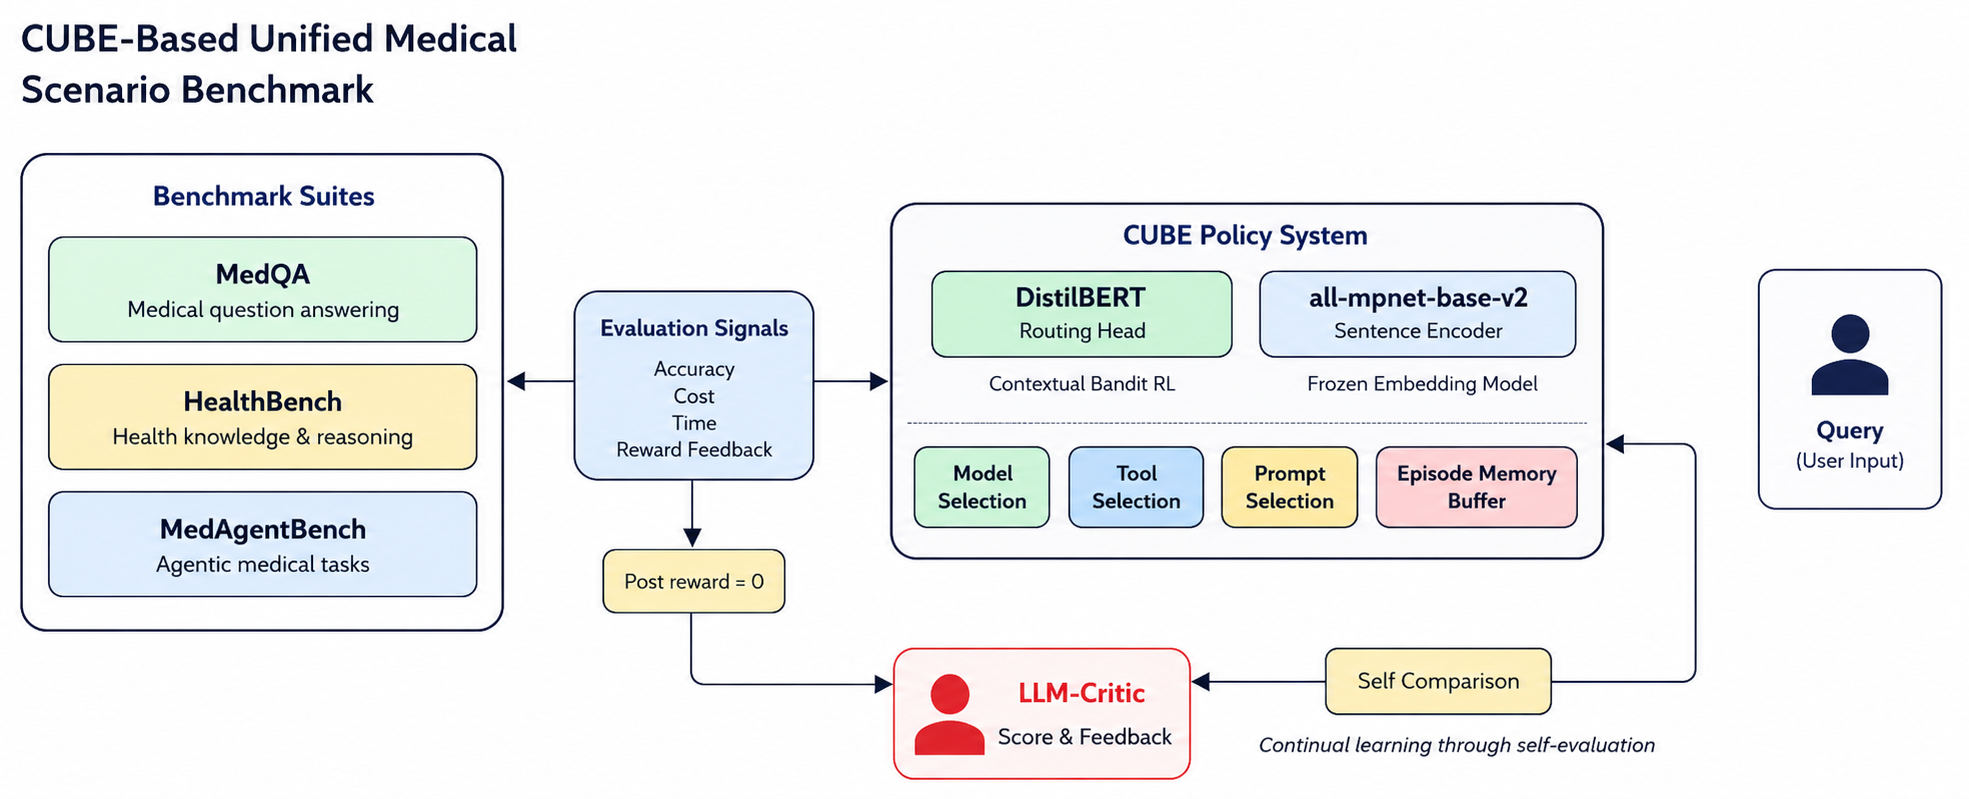
\includegraphics[width=1.0\linewidth]{image.png}
    \caption{A diagram of our proposed approach. A query is passed through a DistilBERT router that classifies to predict preferred model selection, tool selection, and prompt selection. An additional episodic memory mechanism, to retrieve zero reward (failed) memory traces is also presented. }
    \label{fig:system-diagram}
\end{figure}

\begin{table}[htbp]
\centering
\caption{Dataset Split, Inputs, Outputs, and Reward Scoring Across Evaluation Benchmarks}
\label{tab:dataset_details}
\begin{tabular}{|p{1.4cm}|p{0.5cm}|p{1.4cm}|p{1.4cm}|p{2.1cm}|}
\hline
\textbf{Data Split} & \textbf{Total} & \textbf{MMLU-Med} & \textbf{HealthBench} & \textbf{MedAgentBench} \\
\hline
Training & 1,350 & 800 & 400 & 150 \\
\hline
Validation & 450 & 200 & 200 & 50 \\
\hline
Testing & 1,371 & 871 & 400 & 100 \\
\hline
Inputs & & question, \newline choices\_json & messages\_json & instruction, \newline context, \newline tools\_json \\
\hline
Outputs & & QA Answer \newline [A, B, C, D] & Conversation \newline Completion & FHIR database \newline state, \newline Conversation \\
\hline
Reward \newline Scoring & & 0 or 1 (hard \newline coded check) & LLM Response \newline (0 to 1, \newline rubric grade) & LLM Judge \newline (0 or 1, \newline success or fail) \\
\hline
\end{tabular}
\end{table}

\section{Data and Preprocessing}

\subsection{Episodic RAG}

During training run evaluations, failed episodes were recorded as memory candidates. Each text contains the benchmark, task id, reward, failure mode, generic benchmark-specific advice, original task request, model prediction summary, judge/scorer feedback and transcript excerpts. Text is chunked by recursive character splitting, using a chunk boundary of 900 characters with overlap of 120 characters. Chunks are embedded using \texttt{sentence-transformers/all-mpnet-base-v2}, and on evaluation, we use top-3 retrieval using cosine similarity.

\subsection{Routing Dataset}

The training dataset for the routing model was prepared by mapping model queries to model labels, binary tool enablement, and prompt labels (benchmark scenarios).  

Queries were assembled using context from each benchmark:

\begin{lstlisting}[language=python, caption={Prompt assembly}, label=lst:not-available]

Task:
...

Context:
...

Answer options:
...

\end{lstlisting}

The structure of the prompt admittedly made classification easy from content shape. Multiple-choice questions have answer options, MedAgentBench has chart-like context plus operational instructions, and HealthBench has free-form user conversation and request text.

\section{Experimental Design}

distilbert-base-uncased was used as the base architecture, in which we attached a basic head to classify our target labels. The training workflow runs across 4 epochs with an optimized mini-batch size of 32. Weights are updated via an AdamW optimizer using a set learning rate of $2\times10^{-5}$. Table~\ref{tab:model_hyperparameters} and Table~\ref{tab:splitting_parameters} document the hyperparameters.

\begin{table}[htbp]
\centering
\caption{Hyperparameter Configuration for Model Training}
\label{tab:model_hyperparameters}
\begin{tabular}{|l|l|}
\hline
\textbf{Parameter} & \textbf{Value} \\
\hline
Base Model Architecture & distilbert/distilbert-base-uncased \\
\hline
Total Training Epochs & 4 \\
\hline
Mini-Batch Size & 32 \\
\hline
Learning Rate Optimizer & 2e-5 \\
\hline
\end{tabular}
\end{table}

\begin{table}[htbp]
\centering
\caption{Configuration Parameters for Text Splitting}
\label{tab:splitting_parameters}
\begin{tabular}{|l|l|}
\hline
\textbf{Parameter} & \textbf{Value} \\
\hline
Chunk Size Limit & 900 characters \\
\hline
Chunk Overlap Boundary & 120 characters \\
\hline
Split Processing Style & Recursive Character Splitting \\
\hline
\end{tabular}
\end{table}

\subsection{Prompt techniques and LLM-as-a-Judge Queries}

\begin{lstlisting}[language=Python, caption={System and User zero-shot QA prompt}, label=lst:medical_prompt_1]
[
    {
        "role": "system",
        "content": (
            "You are a medical expert. Return ONLY valid JSON in this exact format: "
            "{\"answer\":\"A\",\"confidence\":0.0}. The answer must be A, B, C, or D."
        ),
    },
    {"role": "user", "content": body},
]
\end{lstlisting}

\begin{lstlisting}[language=Python, caption={Judge Prompt for HealthBench Item Rubric Grading}, label=lst:medical_prompt_3]
Your job is to look at a conversation and a rubric item, and score the last turn (i.e., the last assistant response, or the completion) on compliance.
Return a json object with fields: "explanation" and "criteria_met".
[... standard structural guidelines and examples embedded here ...]
\end{lstlisting}

\begin{lstlisting}[language=Python, caption={MedAgentBench API Prompts}, label=lst:medical_prompt_4]
You are an expert in using FHIR functions to assist medical professionals. Based on the question, make one or more tool calls. Format rules:
1. GET url?param_name1=param_value1...
2. POST url [payload data in JSON]
3. FINISH([answer1, answer2, ...])
\end{lstlisting}

\begin{lstlisting}[language=Python, caption={MedAgentBench LLM-as-a-Judge}, label=lst:medical_prompt_5]
[
    {
        "role": "system",
        "content": (
            "You are judging a MedAgentBench task. Compare the model's FINISH payload "
            "against expected outputs. Return JSON with keys: score, success, explanation."
        ),
    }
]
\end{lstlisting}

\section{Experimental Results}

Table~\ref{tab:model_evaluation} outlines our initial QA trials. We were able to compare frontier model capabilities and observationally we measured cost. Notably, though gemini-3-flash outperforms on all tests, all models were comparable had close scores for MMLU-Medical, which inspired us to use it as our QA subset in our unified benchmark, as gpt-oss-120b is measurably faster and cheaper for evaluation.

\begin{table}[htbp]
\centering
\caption{Model Performance Evaluation Across Medical Benchmarks}
\label{tab:model_evaluation}
\begin{tabular}{|p{1.7cm}|l|c|c|c|}
\hline
\textbf{Evaluation} & \textbf{Model} & \textbf{Accuracy} & \textbf{F1-Macro} & \textbf{ECE} \\
\hline
MedQA & gemini-flash-prev & 0.9442 & 0.9438 & 0.0332 \\
MedQA & gemma-4-31b-it & 0.8409 & 0.8394 & 0.1344 \\
MedQA & gpt-oss-120b & 0.9018 & 0.9060 & 0.0632 \\
\hline
MedMCQA & gemini-flash-prev & 0.8505 & 0.8499 & 0.1047 \\
MedMCQA & gemma-4-31b-it & 0.7496 & 0.7475 & 0.2104 \\
MedMCQA & gpt-oss-120b & 0.7352 & 0.7377 & 0.1923 \\
\hline
PubMedQA & gemini-flash-prev & 0.8048 & 0.6238 & 0.1443 \\
PubMedQA & gemma-4-31b-it & 0.7940 & 0.5901 & 0.1709 \\
PubMedQA & gpt-oss-120b & 0.6680 & 0.5800 & 0.2241 \\
\hline
MMLU-Med & gemini-flash-prev & 0.9221 & 0.9198 & 0.0483 \\
MMLU-Med & gemma-4-31b-it & 0.8938 & 0.8914 & 0.0868 \\
MMLU-Med & gpt-oss-120b & 0.8859 & 0.8866 & 0.0819 \\
\hline
\end{tabular}
\end{table}

Table~\ref{tab:rag_evaluation} shows the impact of introducing MedRAG chunks and FAISS, which measurably reduced performance. This is indicative that naive RAG simply adds noise to model QA when imprecise, as we did not carefully optimize it.

\begin{table}[htbp]
\centering
\caption{Performance Comparison of gpt-oss-120b With and Without RAG Across Medical Benchmarks}
\label{tab:rag_evaluation}
\begin{tabular}{|p{2.2cm}|c|c|c|}
\hline
\textbf{Evaluation Domain} & \textbf{Accuracy} & \textbf{F1-Macro} & \textbf{ECE} \\
\hline
MedQA Baseline & 0.9018 & 0.9060 & 0.0632 \\
MedQA With RAG & 0.8995 & 0.9019 & 0.0612 \\
\hline
MedMCQA Baseline & 0.7352 & 0.7377 & 0.1923 \\
MedMCQA With RAG & 0.7322 & 0.7333 & 0.1925 \\
\hline
PubMedQA Baseline & 0.6680 & 0.5800 & 0.2241 \\
PubMedQA With RAG & 0.6440 & 0.5544 & 0.2413 \\
\hline
MMLU-Medical Baseline & 0.8859 & 0.8866 & 0.0819 \\
MMLU-Medical With RAG & 0.8862 & 0.8868 & 0.0773 \\
\hline
\end{tabular}
\end{table}

Table~\ref{tab:test_split_evaluation_base} shows our initial test split evaluation performance, and Table~\ref{tab:train_split_evaluation} shows our scores while preparing training samples for episodic memory data preparation. We get state of the art performance of MMLU-Medical and MedAgentBench, while HealthBench struggles. We can notice that the LLM-as-a-Judge system for HealthBench is also significantly expensive, but is the most robust guardrailing metric.

\begin{table}[htbp]
\centering
\caption{Test Split Base Performance Evaluation Results (Run 1 of 2)}
\label{tab:test_split_evaluation_base}
\begin{tabular}{p{1.4cm} p{1.6cm} c c c c}
\toprule
\textbf{Model} & \textbf{Benchmark} & \textbf{Mean} & \textbf{Latency} & \textbf{Cost} & \textbf{Tokens} \\
\midrule
gemini-3-flash & mmlu medical & 0.9265 & 1.36s & \$0.0831 & 117,420 \\
               & healthbench   & 0.3868 & 26.15s & \$5.8573 & 8,394,373 \\
               & medagentbench & 0.8800 & 5.80s & \$0.5742 & 1,058,002 \\
\bottomrule
\end{tabular}
\end{table}

\begin{table}[htbp]
\centering
\caption{Train Split Evaluation Results across Different Benchmarks}
\label{tab:train_split_evaluation}
\begin{tabular}{p{1.4cm} p{1.6cm} c c c c}
\toprule
\textbf{Model} & \textbf{Benchmark} & \textbf{Mean} & \textbf{Latency} & \textbf{Cost} & \textbf{Tokens} \\
\midrule
gemini-3-flash & mmlu medical & 0.9200 & 1.24s & \$0.0771 & 108,904 \\
               & healthbench  & 0.3778 & 26.06s & \$5.5574 & 7,927,822 \\
               & medagentbench & 0.8667 & 6.24s & \$0.6957 & 1,660,208 \\
\bottomrule
\end{tabular}
\end{table}

The classification accuracy of our trained routing gate layer across the validation and test datasets is documented in Table~\ref{tab:split_evaluation}.

\begin{table}[htbp]
\centering
\caption{Classifier Performance Evaluation Across Data Splits}
\label{tab:split_evaluation}
\begin{tabular}{|l|c|c|c|c|}
\hline
\textbf{Split} & \textbf{n} & \textbf{Model Intent} & \textbf{Tool Routing} & \textbf{Scenario Match} \\
\hline
Train & 1,350 & 99.93\% & 100.00\% & 99.85\% \\
Validation & 450 & 100.00\% & 100.00\% & 100.00\% \\
Test & 1,371 & 99.93\% & 100.00\% & 99.93\% \\
\hline
\end{tabular}
\end{table}

The latency introduced by using the router on a consumer-grade CPU is shown Table~\ref{tab:latency_metrics}, comparing routing and memory retrieval components. We can see that either operation is very cheap even on the edge, and contributes to significant cost savings.

\begin{table}[htbp]
\centering
\caption{Latency Metrics across Different Functional Modes}
\label{tab:latency_metrics}
\begin{tabular}{p{2.3cm} c c c c c}
\toprule
\textbf{Mode} & \textbf{Mean} & \textbf{Median} & \textbf{P95} & \textbf{P99} & \textbf{Max} \\
\midrule
Router only & 99 ms & 85 ms & 196 ms & 273 ms & 530 ms \\
Router component & 162 ms & 158 ms & 257 ms & 331 ms & 392 ms \\
Memory retrieval & 208 ms & 180 ms & 390 ms & 609 ms & 844 ms \\
Combined & 370 ms & 332 ms & 635 ms & 959 ms & 1174 ms \\
\bottomrule
\end{tabular}
\end{table}

Finally, Table*~\ref{tab:test_split_evaluation} shows all evaluations across both our unrouted, gemini-3-flash-preview baseline, and our routed system. We can see reduced costs in both latency and API costs

\begin{table*}[htbp]
\centering
\caption{Test Split Evaluation Results across Different Benchmarks}
\label{tab:test_split_evaluation}
\begin{tabular}{llcccccccc}
\toprule
\textbf{Model Config} & \textbf{Benchmark} & \textbf{Official} & \textbf{Judge} & \textbf{Response} & \textbf{Judge} & \textbf{Response} & \textbf{Judge} & \textbf{Response} & \textbf{Judge} \\
 & & \textbf{score mean} & \textbf{mean} & \textbf{Latency} & \textbf{Latency} & \textbf{Cost} & \textbf{Cost} & \textbf{Tokens} & \textbf{Tokens} \\
\midrule
gemini-3-flash & mmlu\_medical & 0.9242 & --- & 1.274s & --- & \$0.0837 & --- & 117,531 & --- \\
 & healthbench & 0.3907 & --- & 10.231s & 17.935s & \$0.8118 & \$5.0383 & 329,681 & 8,049,743 \\
 & medagentbench & 0.2900 & 0.8600 & 4.075s & 1.947s & \$0.4012 & \$0.0386 & 1,020,350 & 37,337 \\
\midrule
Routed Network & mmlu\_medical & 0.8840 & --- & 0.501s & --- & \$0.0000 & --- & 348,477 & --- \\
 & healthbench & 0.3789 & --- & 11.367s & 23.083s & \$0.7756 & \$5.5229 & 420,002 & 9,179,169 \\
 & medagentbench & 0.3548 & 0.7957 & 2.902s & 1.626s & \$0.3012 & \$0.0322 & 952,973 & 31,534 \\
\midrule
Routed + Memory & mmlu\_medical & 0.8829 & --- & 0.605s & --- & \$0.0003 & --- & 750,067 & --- \\
 & healthbench & 0.3615 & --- & 10.735s & 22.548s & \$0.7602 & \$6.2883 & 551,179 & 10,629,937 \\
 & medagentbench & 0.2000 & 0.8111 & 3.053s & 1.606s & \$0.3317 & \$0.0328 & 1,039,319 & 31,972 \\
\bottomrule
\end{tabular}
\end{table*}

\section{Discussion and Limitations}

As indicated by Table~\ref{tab:split_evaluation}, the fine-tuned intent gate achieved near-perfect classification performance. Though this was likely due to admittedly easy prompting structures, it reveals that even small language models are capable of routing evaluation queries for cost saving and optimization. Basic accuracy was preserved while latency and costs were reduced. 

Our episodic memory lookup system was not successful. Our injected prompts caused a slight degradation in accuracy across benchmarks. Additionally, combining routing layers with memory vector lookups raises cumulative system latency to a mean of $370$ ms (Max $1174$ ms). While this latency remains manageable for offline processes, it may introduce bottlenecks in real-time conversational clinical applications as conversations continue and build up.

A primary limitation of this work relates to evaluation environment unification. Our unification was not a perfect representation of a messy and hard-to-distinguish query system, making our classifier task deceptively easy. 

\section{Conclusions}

This work confirms the feasibility of constructing unified, multi-scenario routing gates across disparate medical evaluation frameworks. We demonstrated that clinical queries can be categorized with high accuracy, minimizing unnecessary inference costs on massive frontier models without significantly degrading accuracy. Our experiments demonstrate that adding context-augmented memory paths does not universally improve task scores and can occasionally distract reasoning models while increasing system latency. Future research will explore creating a more robust unification framework and improvement the unified scenario environment.

\bibliographystyle{IEEEtran}
\bibliography{references}

\end{document}